\documentclass[11pt]{article}
\usepackage[scaled=0.92]{helvet}
\usepackage{geometry}
\geometry{letterpaper,tmargin=1in,bmargin=1in,lmargin=1in,rmargin=1in}
\usepackage[parfill]{parskip} % Activate to begin paragraphs with an empty line rather than an indent %\usepackage{graphicx}
\usepackage{amsmath,amssymb, mathrsfs, dsfont}
\usepackage{tabularx}
\usepackage[font=footnotesize,labelfont=bf]{caption}
\usepackage{graphicx}
\usepackage{xcolor}
%\usepackage[linkbordercolor ={1 1 1} ]{hyperref}
%\usepackage[sf]{titlesec}
\usepackage{natbib}
\usepackage{../../Tianpei_Report}
%\usepackage{appendix}
%\usepackage{algorithm}
%\usepackage{algorithmic}

%\renewcommand{\algorithmicrequire}{\textbf{Input:}}
%\renewcommand{\algorithmicensure}{\textbf{Output:}}



\begin{document}
\title{self-study: Gradient Boost Trees and XGBoost}
\author{ Tianpei Xie}
\date{ Jun. 24th., 2022 }
\maketitle
\allowdisplaybreaks
\section{Boosting}
The basic idea of \emph{\textbf{boosting}} is to combine multiple \textit{weak} learners in sequential manner in order to boost the performance of joint model. Boosting belongs to Generalized Additive Models

\begin{align*}
y &= \sum_{j=1}^{p}f_j(\mb{x}_{i}) + \epsilon
\end{align*} where $f_{j}: \bR^{d} \rightarrow \bR$ or $f_{j}: \bR^{d} \rightarrow \set{0, 1}$ are classifiers belong to a family of simple functions $\cF$. Similar to classical Fourier transform, each $f_{j}$ are able to capure a simple relationship between covariate variables and the response variables, but combining them together, the model is expected to cover both broad and detailed aspects of the target distribution. Boosting belongs to \textit{Ensemble Methods}, which all seeks to improve the performance of machine learning model by joining multiple models together. 

\section{Tree-based methods}
In most of applications for boosting methods, the basis function class $\cF$ is the family of \textbf{tree-based models}.  A tree-based model can be represented as weighted sum of region indicators: 
\begin{align*}
f_{\cT}(\mb{x}) &= \sum_{m=1}^{T}w_{m}\ind{\mb{x} \in \cR_{m}}
\end{align*} where $\cR_{m}$ is the region in $\cR^{k}$ partioned according to a binary tree $\cT$.The partition $\set{\cR_{m}, m=1,\dots,T}$ is generated by branching at one input feature $x^{j}$ at a time. Each \textbf{terminal point} or \textbf{leaves} of the tree represent a partitioned regin.  Tree-based ensemble is a piece-wise constant function,  therefore the class of ensemble trees can also be represented as
\begin{align*}
\cF &\equiv \set{ f_{ \cT}(\mb{x}) = \mb{w}_{q(\mb{x})}: q \in \cT, \forall  \cT  }
\end{align*} where $q: \bR^{d} \rightarrow {1,2,\dots,T}$ is the tree-structured mapping that maps input data to a region index and $\mb{w} = \brac{w_{1}, \dots, c_{T}} \in \bR^{T}$. Given the region partitions $\cR_{m}$,  $c_{m}$ is easy to inference by simpling taking the mean of the target for samples in the region in \textbf{regression tree} or by taking the misclassification error or cross entropy in \textbf{classification tree}.

Note that tree-based ensemble did partition the input space into several regions similar to clustering, but the partition is selected to optimize the loss with respect to target $y$, while for the clustering method the partition is selected to optimize some metrics on the input data $\mb{x}$. There are several advantages when using tree-based methods \citep{hastie2009elements}:
\begin{itemize}
\item Making predictions is \textbf{fast} (no complicated calculations, just looking up
constants in the tree)
\item It’s easy to understand / \textbf{interpret} what variables are important in making the prediction (look at the tree)
\item If some data is \emph{missing}, we might not be able to go all the way down the
tree to a leaf, but we can still make a prediction by averaging all the leaves
in the sub-tree we do reach
\item The model gives a jagged response, so it can work when the true regression
surface is not smooth. If it is smooth, though, the piecewise-constant
surface can approximate it arbitrarily closely (with enough leaves)
\item There are fast, reliable algorithms to learn these trees
\end{itemize}



Learning a tree ensemble $f$ can be done by optimizing the objective function 
\begin{align*}
\cL(f) &:= \sum_{i}\cL(y_i, \hat{y}_{i}) +\gamma \Omega(\cT) + \frac{\alpha}{2} \norm{\mb{w}}{2}^{2} \\
&= \sum_{m=1}^{T}\sum_{i: \mb{x}_{i} \in \cR_{m}}\cL(y_i, w_{m}) +\gamma \Omega(\cT) + \frac{\alpha}{2}\sum_{m=1}^{T} w_{m}^{2} 
\end{align*}
where $\cL$ is the regression loss function such as mean squared error, $\hat{y}_{i} = f(\mb{x}_{i})$ is the predicted output of the ensemble given i-th sample $\mb{x}_{i}$. The second term  $\Omega(\cdot)$ measure the complexity of the tree $\cT$. The last term is a smoothing factor. Since the objective function is non-smooth, the solution is based on a \emph{\textbf{recursive greedy algorithm in top-down manner}}: 

\begin{itemize}
\item begin with the root node, finding one feature that split the input space into two nodes/regions;
\item in order to find the optimal split, for each region, estimate $w_{j}$ by taking average of responses within the region
\item compute the loss / residual for the esimate in each region; the optimal split is the one tha minimize the objective function
\item for each region, repeat previous steps to further partition
\item stop growing the tree when some criteria are met
\end{itemize}

Usually we can make sure that the tree stop growing when some minimal node size has been reached. When tree grow too large,  we will reduce the tree complexity by using \emph{\textbf{cost-complexity pruning}}. Let $\cT \subset \cT_{0}$ be a tree obtained after prunning $\cT_{0}$, i.e. by collapsing any number of non-terminal nodes (internal nodes) in $\cT_{0}$. Let $\cR_{m}, m=1,\dots,T$ be regions partitioned via terminal nodes. 

For \textbf{regression tree}, we can define cost complexity criterion as 
\begin{align*}
C_{\gamma}(\cT) &= \sum_{m=1}^{T}\sum_{i: \mb{x}_{i} \in \cR_{m}}(y_i - \hat{w}_{m})^{2} + \gamma T
\end{align*} where $\hat{w}_{m} = \frac{1}{|\set{\mb{x}_{i} \in \cR_{m}}|} \sum_{i: \mb{x}_{i} \in \cR_{m}} y_{i}$. $Q_{m}(\cT) := \sum_{i: \mb{x}_{i} \in \cR_{m}}(y_i - \hat{w}_{m})^{2} / N_{m}$ is the variance or residual of the loss \citep{hastie2009elements}.  Then the idea is to find, for each $\gamma$, $\cT_{\lambda} \subseteq \cT_{0}$ to minimize the $C_{\gamma}(\cT)$. $\gamma$ is the tuning parameters which balance the goodness-of-fit and the model complexity. It can be shown that for given $\gamma$ there exists a \emph{unique} tree $\cT_{\gamma}$ that minimize the cost complexity criterion. This solution can be found via \emph{\textbf{weakest link pruning}}: i.e. we successively collaps two internal nodes that produce the smallest per-node increase in residual. We continue this process until we reach out to the root. The process gives us a sequence of trees and the optimal $\cT_{\gamma}$ must exist within this sequence, i.e. the tree that minimize the cost among trees in the sequence is the optimial solution. 

For \textbf{classification tree}, the \emph{residual} $Q_{m}(\cT) := \sum_{i: \mb{x}_{i} \in \cR_{m}}(y_i - \hat{w}_{m})^{2} / N_{m}$ in each region can be replaced by some \emph{impurity measure}. Note that $\hat{p}_{mk} := \sum_{i: \mb{x}_{i} \in \cR_{m}}\ind{y_{i} = k}/ N_{m}$ is the proportion of label $k$ in the region. The classification within the region can be done via majority vote $k_m := \argmax_{k} \hat{p}_{mk}$.  Some commonly used impurity measure are
\begin{itemize}
\item misclassification error: $1-\hat{p}_{mk_{m}} := \sum_{i: \mb{x}_{i} \in \cR_{m}}\ind{y_{i} \neq k_{m}}/ N_{m}$
\item \emph{Gini index}: $\sum_{k \neq k'}\hat{p}_{mk}\hat{p}_{mk'} = \sum_{k}^{K}\hat{p}_{mk}(1-\hat{p}_{mk})$ 
\item cross-entropy: $-\sum_{k=1}^{K}\hat{p}_{mk}\log \hat{p}_{mk}$ 
\end{itemize}
Both cross-entropy and Gini Index are more sensitive to node probabililty change than misclassification error. 

Tree-based methods can handle \emph{missing value} more flexibly. First, it can treat the missing value as additional category in categorical features. This allows us to encode the pattern of missing value itself into the model. Second, it can construct surrogate variables. When considering a predictor for split, we use only observations for which the predictor is not missing. Having choosing the optimal primary predictor and split, we form a list of \emph{surrogate predictors and split points}. The first surrogate is the predictor and corresponding split point that best mimic the split of training data done by the primary predictor. The second is the one secondly best mimic the primary split. Then in prediction phase, let the observations go through the surrogate predictors and splits \emph{in order}. The higher the \textbf{correlation} between missing/primary predictor and surrogate predictors, the smaller the loss of information due to missing value. 

Tree-based methods are known to be of \textbf{higher variance} due to the greedy splits it generates. A small change of data will result in a  different series of splits, making interpretation more precautious. The major reason is due ot the hierarchical nature of the tree-building process: the effect of error in root split will be propagated to all splits below.  Ensemble methods such as boosting will help to reduce the variance for tree-based model. 


\section{Boosting as Forward Stagewise Additive Modeling}
Learning in boosting is done stagewise sequentially. At each stage, a new model $f_{j}$ is learned and added to the ensemble, so that the overall objective is minimized. We can use the following function to define the objective of boosting model:
 \begin{align*}
\cL(f) &:= \sum_{i}\cL\paren{y_i, \hat{y}_{i}} +\gamma  \sum_{j}\Omega(\cT_{j}) + \frac{\alpha}{2} \sum_{j}\norm{\mb{w}_{j}}{2}^{2} \\
&= \sum_{i}\cL\paren{y_i,  \sum_{j=1}^{p}\beta_{j}f_j(\mb{x}_{i})}  +\gamma  \sum_{j}\Omega(\cT_{j}) + \frac{\alpha}{2} \sum_{j}\norm{\mb{w}_{j}}{2}^{2}
\end{align*} where $ \hat{y}_{i} = \sum_{j=1}^{p}f_j(\mb{x}_{i})$ and $f_{j} \in \cF$ of tree ensembles. Then at stage $k$, the objective can be modified as 
 \begin{align}
\cL_{k}(f_{k} | f^{k-1}) &:= \sum_{i}\cL\paren{y_i,  \sum_{j=1}^{k-1}\beta_{j}f_j(\mb{x}_{i}) + \beta_{k}f_{k}(\mb{x}_{i})}  +\gamma  \sum_{j}^{k-1}\Omega(\cT_{j}) + \frac{\alpha}{2} \sum_{j}^{k-1}\norm{\mb{w}_{j}}{2}^{2} \nonumber\\
&= \sum_{i}\cL\paren{y_i, f^{k-1}(\mb{x}_{i}) +\beta_{k} f_{k}(\mb{x}_{i})}  +\gamma  \sum_{j}^{k-1}\Omega(\cT_{j}) + \frac{\alpha}{2} \sum_{j}^{k-1}\norm{\mb{w}_{j}}{2}^{2} \label{eqn: forward_objective}
\end{align} where $f^{k-1}(\mb{x}_{i}) = \sum_{j=1}^{k-1}\beta_{j}f_j(\mb{x}_{i})$ is the ensemble learned at previous stage.

For \textbf{squared loss} $\cL(y,f) := (y-f(x))^2$, the above equation \eqref{eqn: forward_objective} can be represented as 
\begin{align*}
\cL_{k}(f_{k} | f^{k-1}) &= \sum_{i}\paren{y_i - f^{k-1}(\mb{x}_{i}) - \beta_{k} f_{k}(\mb{x}_{i})}^2 \\
&=  \sum_{i}\paren{r_{i,k} - \beta_{k} f_{k}(\mb{x}_{i})}^2 
\end{align*} where $r_{i,k}:= y_i - f^{k-1}(\mb{x}_{i})$ is the \emph{residual} of the ensemble at previous stage at current observation. So for squared loss, the new model $f_{j}$ is learned to be the best fit to the residual of previous ensemble. $ensemble \rightarrow residual \rightarrow new\_ensemble$.

For \textbf{exponential loss} $\cL(y,f) := \exp(-y\,f(x))$, the \eqref{eqn: forward_objective} becomes AdaBoost. 
\begin{align*}
\cL_{k}(f_{k} | f^{k-1}) &= \sum_{i}\exp\paren{-y_i (f^{k-1}(\mb{x}_{i}) + \beta_{k} f_{k}(\mb{x}_{i}))} \\
&=  \sum_{i}\exp\paren{-y_i f^{k-1}(\mb{x}_{i})} \exp\paren{ -y_{i}\beta_{k} f_{k}(\mb{x}_{i})} \\
&=  \sum_{i}D_{i,k-1} \exp\paren{ -y_{i}\beta_{k} f_{k}(\mb{x}_{i})}
\end{align*}

For tree-based model $f$, we can further decompose the equation \eqref{eqn: forward_objective} as 
\begin{align}
\cL_{k}(f_{k} | f^{k-1}) &:=  \sum_{i}\cL\paren{y_i, f^{k-1}(\mb{x}_{i}) +\beta_{k} f_{k}(\mb{x}_{i})} + \Omega(\cT) \nonumber\\
&=  \sum_{m=1}^{T}\sum_{i: \mb{x}_{i} \in \cR_{m}}\cL\paren{y_i, f^{k-1}(\mb{x}_{i}) +\beta_{k}*w_{m} } + \Omega(\cT) \nonumber\\
\cL_{k}(\set{\theta_{k,m}, \cR_{m}} | f^{k-1})&:=  \sum_{m=1}^{T}\sum_{i: \mb{x}_{i} \in \cR_{m}}\cL\paren{y_i, f^{k-1}(\mb{x}_{i}) +\theta_{k,m} } + \Omega(\cT) \label{eqn: forward_objective_tree}
\end{align} Note that the continuous score $\theta_{k,m}$ can be learned by minimizing $$\sum_{i: \mb{x}_{i} \in \cR_{m}}\cL\paren{y_i, f^{k-1}(\mb{x}_{i}) +\theta_{k,m} }$$ within each region $\cR_{m}$. We can choose $\beta_{k} = \beta$ and call it the \textbf{\emph{learning rate}} of boosting algorithm.


\section{Gradient Boost Trees}
The objective function \eqref{eqn: forward_objective} can be \emph{approximated} via its first and second order approximation at $f^{k-1}$. 
\begin{align}
\cL_{k}(f_{k} | f^{k-1}) = \cL_{k}(f) &:\approx  \cL_{k}(f^{k-1}) + \grad{\cL}|_{f^{k-1}}^{T}\;\Delta f + \frac{1}{2}H_{\cL}|_{f^{k-1}} \norm{\Delta f}{2}^2  \nonumber\\
&=   \sum_{i}\cL\paren{y_i, f^{k-1}(\mb{x}_{i})} + \sum_{i}g_{i,k} f_{k}(\mb{x}_{i}) + \frac{1}{2}\sum_{i}h_{i,k} f_{k}^2(\mb{x}_{i}) \nonumber\\
&= const. +  \sum_{i}g_{i,k} f_{k}(\mb{x}_{i}) + \frac{1}{2}\sum_{i}h_{i,k} f_{k}^2(\mb{x}_{i}) \label{eqn: forward_objective_grad} \\
&= const. + \frac{1}{2} \sum_{i}h_{i,k}\paren{f_{k}(\mb{x}_{i}) + \frac{g_{i,k}}{h_{i,k}}}^{2} \label{eqn: forward_objective_grad_weight}
\end{align} where 
\begin{align*}
g_{i,k} &:= \brac{\frac{\partial \cL(y_i, f(\mb{x}_{i}))}{\partial f(\mb{x}_{i})}}_{f=f^{k-1}(\mb{x}_{i})} \\
h_{i,k} &=  \brac{\frac{\partial^2 \cL(y_i, f(\mb{x}_{i}))}{\partial^{2} f(\mb{x}_{i})}}_{f=f^{k-1}(\mb{x}_{i})}
\end{align*} are gradient and Hessian of the loss function w.r.t. functions $f$. Since these methods use gradient approximation to build boosting trees, it is called \emph{\textbf{gradient boost methods}}. Example of loss function and their first and second order derivatives:
\begin{itemize}
\item \textbf{squared loss} $\cL(f) := (y-f)^2 /2$: $g:= (f-y)$, $h := -y$
\item  \textbf{binary cross-entropy loss (logistic loss)} $\cL(f) :=-( y\log(f) + (1-y)\log(1-f))$, $g:= \frac{f-y}{(1- f)f}$ , $h :=\frac{y}{f^2} + \frac{1-y}{(1-f)^2}$
\end{itemize}

For tree-based models, equation \eqref{eqn: forward_objective_grad} can be simplified as
\begin{align}
&\sum_{m=1}^{T}\sum_{i: \mb{x}_{i} \in \cR_{m}}\paren{g_{i,k} w_{m} + \frac{1}{2}h_{i,k} w_{m}^2} +  \Omega(\cT) \nonumber\\
&=\sum_{m=1}^{T}\sum_{i: \mb{x}_{i} \in \cR_{m}}\paren{g_{i,k} w_{m} + \frac{1}{2}h_{i,k} w_{m}^2} + \gamma\,T + \alpha\,\frac{1}{2}\sum_{m=1}^{T}\sum_{i: \mb{x}_{i} \in \cR_{m}} w_{m}^2\nonumber\\
&=\sum_{m=1}^{T}\sum_{i: \mb{x}_{i} \in \cR_{m}}\paren{g_{i,k} w_{m} + \frac{1}{2}(h_{i,k}+\alpha) w_{m}^2} + \gamma\,T.  \label{eqn: forward_objective_grad_tree}
\end{align} So if we fixed the tree structure, i.e. $\cR_{m}, \forall m$, then finding the optimal weight (score) $w_{m}$ can be done easily by minimizing the above equation. We have 
\begin{align}
w_{m}^{*}&:= \argmin_{w_{m}}\sum_{i: \mb{x}_{i} \in \cR_{m}}\paren{g_{i,k} w_{m} + \frac{1}{2}(h_{i,k}+\alpha) w_{m}^2} \nonumber\\
&=\paren{\sum_{i: \mb{x}_{i} \in \cR_{m}}g_{i,k}}w_{m} + \frac{1}{2}\paren{\sum_{i: \mb{x}_{i} \in \cR_{m}}(h_{i,k}+\alpha)}w_{m}^2 \nonumber\\
&= -\frac{\sum_{i: \mb{x}_{i} \in \cR_{m}}g_{i,k}}{\sum_{i: \mb{x}_{i} \in \cR_{m}}(h_{i,k}+\alpha)}  \label{eqn: forward_objective_grad_optimal_weight}
\end{align} and the optimal objective value is 
\begin{align}
\hat{ \cL_{k}}^{*}(f) &= -\frac{1}{2}\sum_{m=1}^{T}\frac{\paren{\sum_{i: \mb{x}_{i} \in \cR_{m}}g_{i,k}}^2}{\sum_{i: \mb{x}_{i} \in \cR_{m}}(h_{i,k}+\alpha)} + \gamma T \label{eqn: grad_boost_score}
\end{align}

Here, we can use the equation \eqref{eqn: grad_boost_score} to measure the \textbf{impurity of the split}. Note that we can measure the impact of the split $\mathcal{I}_{o} = \mathcal{I}_{L}\cup \mathcal{I}_{R}$ via the loss reduction 
\begin{align}
 \frac{1}{2}\brac{  \frac{\paren{\sum_{i\in \mathcal{I}_{L}}g_{i,k}}^2}{\sum_{i\in \mathcal{I}_{L}}(h_{i,k}+\alpha)}  + \frac{\paren{\sum_{i\in \mathcal{I}_{R}}g_{i,k}}^2}{\sum_{i\in \mathcal{I}_{R}}(h_{i,k}+\alpha)} - \frac{\paren{\sum_{i\in \mathcal{I}_{o}}g_{i,k}}^2}{\sum_{i\in \mathcal{I}_{o}}(h_{i,k}+\alpha)}} - \gamma T. \label{eqn: split_find_criteria}
\end{align} This equation \eqref{eqn: split_find_criteria} is used in practice to choose split candidate \citep{chen2016xgboost}.

Gradient boost methods can be seen as searching for \emph{\textbf{gradients in functional space}} $\cF$, since the the optimal solution for a new model $f_{k}$  should fit the \textbf{negative gradient values} of the ensemble $-\mb{g} = -\grad{\cL}|_{f^{k-1}}$. For instance, when the loss function is squared loss, one fits the tree $\cT$ according to the  residual of the ensemble in previous iterations via least square. Both gradient boost methods and the recursive greedy algorithm to fit the tree are appoximation procedures. From \eqref{eqn: forward_objective_grad_weight}, we can see that, similar to AdaBoost, the gradient boost method also reweights samples. Unlike Adaboost, which use the mis-classification error to upweight/downweight samples, the gradient boosting uses the \textbf{curvature of error surface} to upweight/downweight samples.  It \textbf{downweight} samples located in \emph{flat} surface and \textbf{upweight} the samples reside in \textbf{\emph{steep curvature}} of the error surface. 
\begin{figure}
\begin{minipage}[t]{1\linewidth}
  \centering
  \centerline{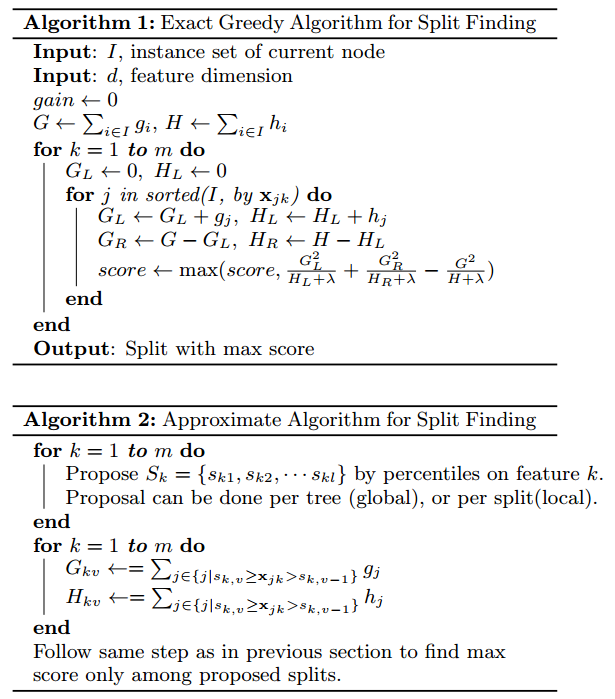
\includegraphics[scale = 0.5]{split_algo.png}}
\end{minipage}
\caption{\footnotesize{\textbf{Split finding algorithm}. The exact split finding algorithm search all featues and sort the data according to feature value. It then accumulate gradient statistics for the structure score in \eqref{eqn: split_find_criteria}. \citep{chen2016xgboost}}}
\label{fig: split}
\end{figure}
\subsection{Split finding algorithm}
One of the key problems in tree learning is to find the best split as indicated in \eqref{eqn: split_find_criteria}. There are two ways to find it: the \textbf{exact greedy search} and the \textbf{approximate greedy search}. In exact greedy search, one enumerates all possible split for all continous features. In order to do so efficiently, the algorithm must first \emph{\textbf{sort}} the data according to feature values and visit the data in sorted order to \emph{accumulate} the gradient statistics for the structure score in \eqref{eqn: split_find_criteria}. The drawbacks for exact greedy search is that it needs to fit all data into the memory. It is not efficient for distributed computing as well. In order to support these two settings, the appoximate greedy search is proposed. See figure \ref{fig: split} for descriptions of the algorithms.

The appoximate greedy search first propose a set of candidate splitting points based on the \textbf{percentiles} of feature distribution. The algorithm then maps the continous features into the \textbf{buckets} defined by these spiltting point, aggregates statistics and find the optimal solution based on the aggregated statistics. There are two \emph{variants}: \textbf{global approximate} or \textbf{local approximate}. The global approximate proposes all candidates at the intital step of tree construction and uses the same proposal for split finding for all levels below. The local approximate re-proposes candidates after each split. The global method requires less proposal steps than the local method. However, usually more candidate points are needed for the global proposal because candidates are not refined after each split. The local proposal refines the candidates after splits, and can potentially be more appropriate for deeper trees \citep{chen2016xgboost}.

The appoximate greedy search use the percentile of feature distribution to find candidte split points. A \emph{\textbf{weighted}} quantile is proposed in \citep{chen2016xgboost} to improve this procedure. Let $(x_{i,d}, h_{i})$ be the sample-hessian pair, where $x_{i,d}$ be the feature $d$ for $i$-th sample and $h_{i}$ is the second-order derivatives for the loss w.r.t. $f$. For all sample-hessian pair of feature $d$ in training set as $\cD_{d} := \brac{(x_{i,d}, h_{i})}_{i}$. We can define a rank function $r_{d}: \cR \rightarrow [0,\infty)$:
\begin{align*}
r_{d}(t) &:= \frac{\sum_{i: x_i < t}h_{i}}{\sum_{i}h_{i}}.
\end{align*} It measures the propotion of instances whose feature $d$ is less than $t$, \textbf{weighted by second-order derivatives} $h_{i}$ at sample $i$. We then find the candidate split points as $[s_{0,d}, \ldots, s_{l,d}]$ where $s_{0,d} = \min_{i}x_{i,d}$ and $s_{l,d} = \max_{i}x_{i,d}$ and $|s_{i,d} - s_{i+1,d}| <= \epsilon$ whiich split the interval between min and max of feature value into $l$ buckets, each size no greater than $\epsilon$. The reason weighted by $h_{i}$ is that the approximate in \eqref{eqn: forward_objective_grad} can be seen as quadratic form $h_{i}(f + g_{i}/h_{i})^2$.  

\section{XGBoost}
XGBoost \citep{chen2016xgboost} is an open source package for the gradient boosting tree algorithm. It has been popular among industry and competitions. XGBoost provides additional optimization on the gradient boosting algorithm to make is successful in real data.

\textbf{\emph{Features}} of XGBoost:
\begin{itemize}
\item Support both single and \textbf{distributed systems}(Hadoop, Spark). As discussed above, XGBoost use global/local approximate split finding algorithm to handle distributed data. It also stores data in blocks and compressed columns. 
\item XGBoost is used in supervised learning(regression and classification problems). Due to generic setting on gradient boosting, it can be used with cross-entropy loss, squared loss etc.
\item Supports \textbf{parallel processing}. It compressed data in each column and stored samples separately in in-memory \emph{blocks} (a.k.a. \emph{\textbf{column blocks}} since each column store the value of features). Data in blocks can be reused and distributed via multiple machines. In approximate split finding, using \emph{sorted data structure} within each blocks, only linear scan is needed. Morever, collecting statstics in \eqref{eqn: split_find_criteria} can be paralleled too since each column is treated independently. 
\item \textbf{Column subsampling}. Similar to Random Forest, XGBoost can select a subset of features in each block/batch to reduce the variance and to prevent overfitting.
\item Cache optimization. While the proposed block structure helps optimize the computation complexity of split finding, the new algorithm requires indirect fetches of gradient statistics by row index, since these values are accessed in order of feature. This is a non-continuous memory access.For the exact greedy algorithm, we can alleviate the problem by a \textbf{cache-aware prefetching algorithm}. For approximate algorithms, we solve the problem by choosing a correct block size. 
\item Efficient memory management for large datasets exceeding RAM. It uses techniques such as \textbf{block compression} and \textbf{block sharding}. 
\item Has a variety of regularizations which helps in reducing overfitting. For example, XGBoost uses \textbf{shrinkage} to scale down newly added weights by a factor $\eta$ after each step of tree boosting. $\eta$ is called the \emph{learning rate}. 
\item Auto tree pruning – Decision tree will not grow further after certain limits internally. Using the criteria defined in \eqref{eqn: grad_boost_score}.
\item Can handle \textbf{missing values}. It implements \textbf{sparsity-aware split finding}. See Figure \ref{fig: sparse_split}.  There are multiple possible causes for sparsity: 1) presence of missing values in the data; 2) frequent zero entries in the statistics; and, 3) artifacts of feature engineering such as one-hot encoding. In order to handle sparsity, a default direction is computed. When
a value is missing in the sparse matrix $X$, the instance is classified into the default direction. There are two choices of default direction at each branch, and the optimal default directions are learned from the data. Finally, only \textbf{non-missing entries} are visited to define buckets. 
\item Has inbuilt Cross-Validation.
\item Takes care of outliers to some extent. Because it uses weighted quantile for each feature in appoximate split finding, the rare extreme values does not affect the split candidate proposals.  
\end{itemize}

\begin{figure}
\begin{minipage}[t]{1\linewidth}
  \centering
  \centerline{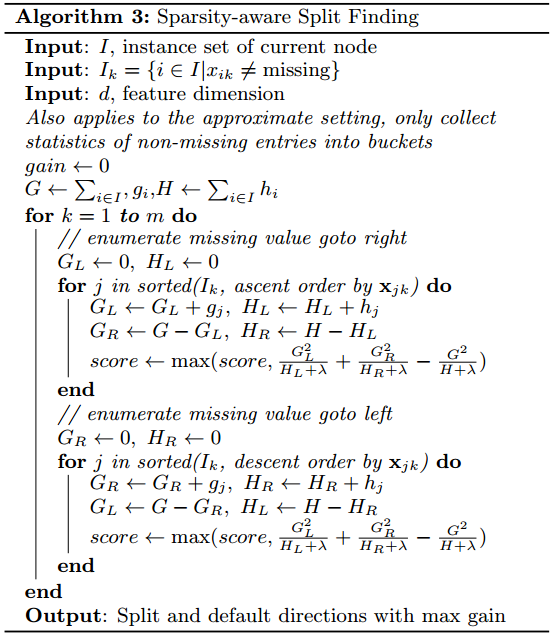
\includegraphics[scale = 0.5]{sparsity_split.png}}
\end{minipage}
\caption{\footnotesize{\textbf{Sparsity-aware split finding algorithm}. The approximate split finding algorithm only the non-missing entries and search for different choice of default directions at each branch. \citep{chen2016xgboost}}}
\label{fig: sparse_split}
\end{figure}

\newpage
\bibliographystyle{plainnat}
\bibliography{book_reference.bib}
\end{document}